\documentclass[tikz,border=10pt]{standalone}
\usetikzlibrary{arrows.meta,backgrounds,calc}
\definecolor{route}{RGB}{31,78,121}
\definecolor{corefill}{RGB}{233,239,247}
\definecolor{outside}{RGB}{120,120,120}
\begin{document}
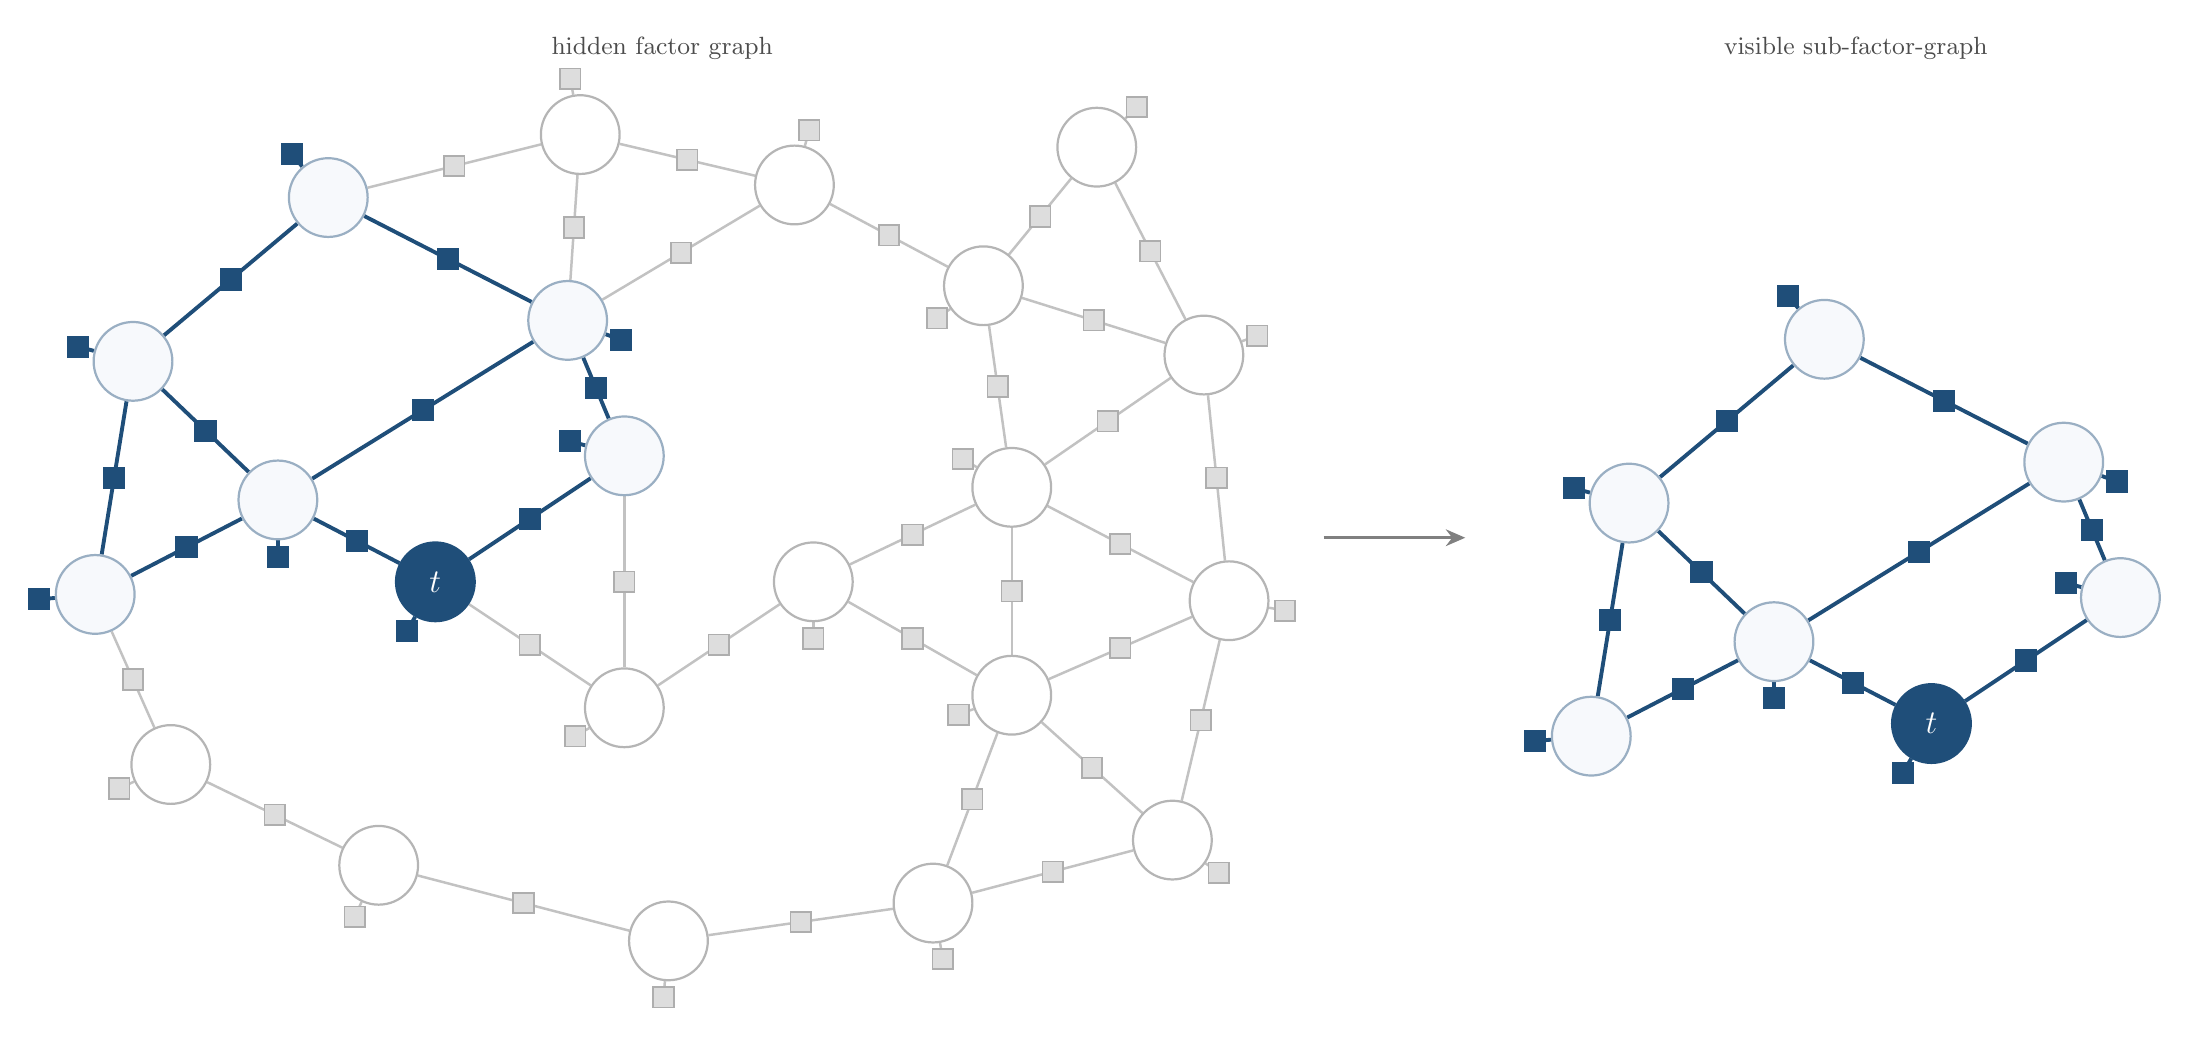
\begin{tikzpicture}[
  >={Stealth[length=7pt,width=6pt]},
  var/.style={circle,minimum size=1.0cm,inner sep=0pt,font=\large,line width=0.8pt},
  seen/.style={var,draw=route!45,fill=white!65!corefill},
  target/.style={var,draw=route,fill=route,text=white},
  hidden/.style={var,draw=outside!55,fill=white,text=outside},
  fac/.style={rectangle,minimum size=0.26cm,inner sep=0pt,line width=0.6pt},
  seenfac/.style={fac,draw=route,fill=route},
  hiddenfac/.style={fac,draw=outside!60,fill=outside!25},
  seenedge/.style={route,line width=1.4pt},
  hiddenedge/.style={outside!45,line width=0.9pt},
  vlabel/.style={font=\large,text=route,inner sep=2pt},
  title/.style={font=\small,text=black!70}
]
\newcommand{\pairfac}[3]{\draw[#1edge] (#2)--(#3);\node[#1fac] at ($(#2)!0.5!(#3)$) {};}
\newcommand{\unfac}[3]{\draw[#1edge] (#2)--++(#3:0.72);\node[#1fac] at ($(#2)+(#3:0.72)$) {};}
% ================= left: hidden factor graph =================
\begin{scope}[shift={(0.000,0.000)}]
\node[target] (t) at (0.000,0.000) {$t$};
\node[seen] (a) at (2.400,1.600) {};
\node[hidden] (b) at (2.400,-1.600) {};
\node[hidden] (c) at (4.800,0.000) {};
\node[seen] (w) at (-2.000,1.040) {};
\node[seen] (x) at (1.680,3.320) {};
\node[hidden] (y) at (7.320,1.200) {};
\node[hidden] (z) at (7.320,-1.440) {};
\node[seen] (p1) at (-4.320,-0.160) {};
\node[seen] (p2) at (-3.840,2.800) {};
\node[seen] (p3) at (-1.360,4.880) {};
\node[hidden] (p4) at (1.840,5.680) {};
\node[hidden] (p5) at (4.560,5.040) {};
\node[hidden] (p6) at (6.960,3.760) {};
\node[hidden] (p7) at (9.760,2.880) {};
\node[hidden] (p8) at (10.080,-0.240) {};
\node[hidden] (p9) at (9.360,-3.280) {};
\node[hidden] (p10) at (6.320,-4.080) {};
\node[hidden] (p11) at (2.960,-4.560) {};
\node[hidden] (p12) at (-0.720,-3.600) {};
\node[hidden] (p13) at (-3.360,-2.320) {};
\node[hidden] (p14) at (8.400,5.520) {};
\begin{scope}[on background layer]
\pairfac{seen}{t}{a}
\pairfac{hidden}{t}{b}
\pairfac{hidden}{a}{b}
\pairfac{hidden}{b}{c}
\pairfac{seen}{t}{w}
\pairfac{seen}{a}{x}
\pairfac{hidden}{c}{y}
\pairfac{hidden}{c}{z}
\pairfac{seen}{w}{x}
\pairfac{hidden}{y}{z}
\pairfac{seen}{w}{p1}
\pairfac{seen}{w}{p2}
\pairfac{seen}{p1}{p2}
\pairfac{seen}{x}{p3}
\pairfac{seen}{p2}{p3}
\pairfac{hidden}{x}{p4}
\pairfac{hidden}{p3}{p4}
\pairfac{hidden}{p4}{p5}
\pairfac{hidden}{x}{p5}
\pairfac{hidden}{y}{p6}
\pairfac{hidden}{p5}{p6}
\pairfac{hidden}{p6}{p7}
\pairfac{hidden}{y}{p7}
\pairfac{hidden}{y}{p8}
\pairfac{hidden}{z}{p8}
\pairfac{hidden}{p7}{p8}
\pairfac{hidden}{z}{p9}
\pairfac{hidden}{p8}{p9}
\pairfac{hidden}{z}{p10}
\pairfac{hidden}{p9}{p10}
\pairfac{hidden}{p10}{p11}
\pairfac{hidden}{p11}{p12}
\pairfac{hidden}{p12}{p13}
\pairfac{hidden}{p1}{p13}
\pairfac{hidden}{p6}{p14}
\pairfac{hidden}{p7}{p14}
\unfac{seen}{t}{240}
\unfac{seen}{a}{165}
\unfac{hidden}{b}{210}
\unfac{hidden}{c}{270}
\unfac{seen}{w}{270}
\unfac{seen}{x}{340}
\unfac{hidden}{y}{150}
\unfac{hidden}{z}{200}
\unfac{seen}{p1}{185}
\unfac{seen}{p2}{165}
\unfac{seen}{p3}{130}
\unfac{hidden}{p4}{100}
\unfac{hidden}{p5}{75}
\unfac{hidden}{p6}{215}
\unfac{hidden}{p7}{20}
\unfac{hidden}{p8}{350}
\unfac{hidden}{p9}{325}
\unfac{hidden}{p10}{280}
\unfac{hidden}{p11}{265}
\unfac{hidden}{p12}{245}
\unfac{hidden}{p13}{205}
\unfac{hidden}{p14}{45}
\end{scope}
\end{scope}
\node[title] at (2.880,6.780) {hidden factor graph};
\draw[->,line width=1.2pt,black!50] (11.280,0.560) -- (13.080,0.560);
% ================= right: induced sub-factor-graph =================
\begin{scope}[shift={(19.000,-1.800)}]
\node[target] (rt) at (0.000,0.000) {$t$};
\node[seen] (ra) at (2.400,1.600) {};
\node[seen] (rw) at (-2.000,1.040) {};
\node[seen] (rx) at (1.680,3.320) {};
\node[seen] (rp1) at (-4.320,-0.160) {};
\node[seen] (rp2) at (-3.840,2.800) {};
\node[seen] (rp3) at (-1.360,4.880) {};
\begin{scope}[on background layer]
\pairfac{seen}{rt}{ra}
\pairfac{seen}{rt}{rw}
\pairfac{seen}{ra}{rx}
\pairfac{seen}{rw}{rx}
\pairfac{seen}{rw}{rp1}
\pairfac{seen}{rw}{rp2}
\pairfac{seen}{rp1}{rp2}
\pairfac{seen}{rx}{rp3}
\pairfac{seen}{rp2}{rp3}
\unfac{seen}{rt}{240}
\unfac{seen}{ra}{165}
\unfac{seen}{rw}{270}
\unfac{seen}{rx}{340}
\unfac{seen}{rp1}{185}
\unfac{seen}{rp2}{165}
\unfac{seen}{rp3}{130}
\end{scope}
\end{scope}
\node[title] at (18.040,6.780) {visible sub-factor-graph};
\end{tikzpicture}
\end{document}
